\documentclass[border=5mm]{standalone}
\usepackage{pgfplots}
\pgfplotsset{compat=1.18}

\begin{document}
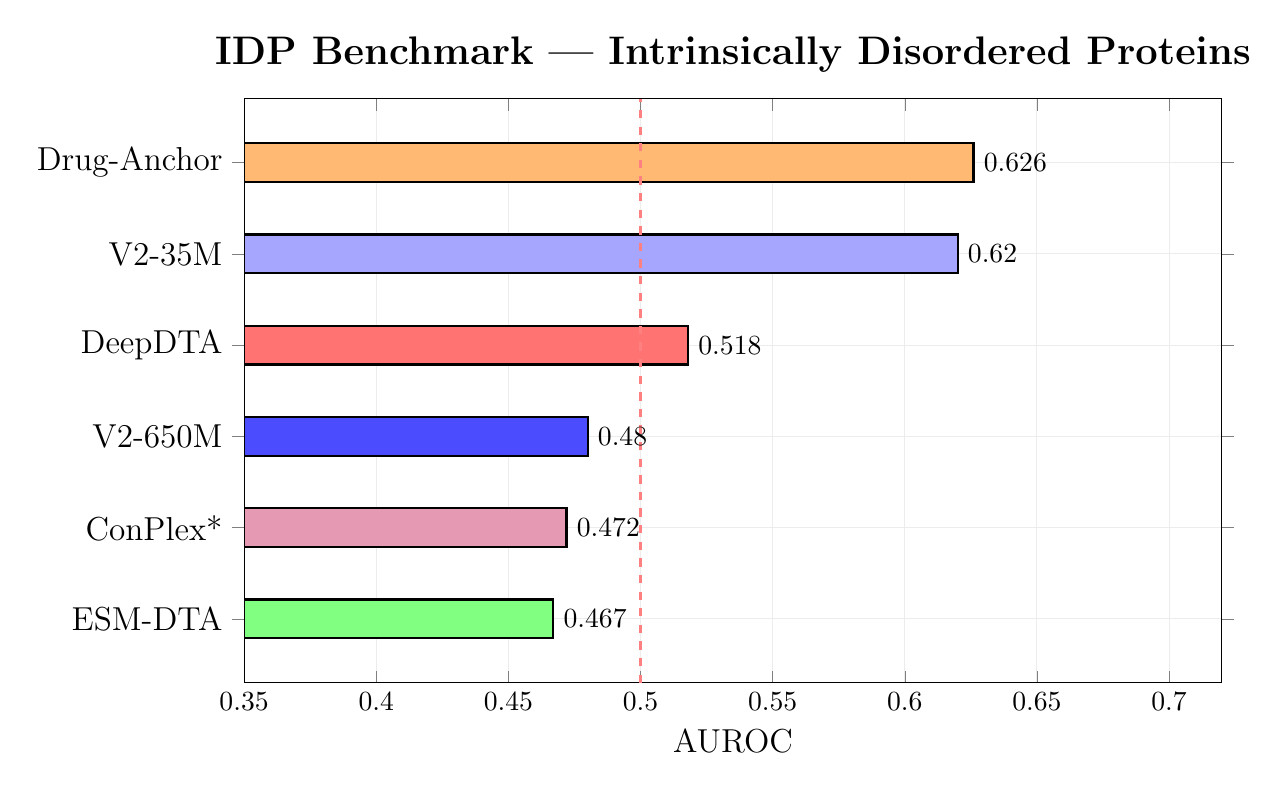
\begin{tikzpicture}
\begin{axis}[
    xbar,
    bar width=14pt,
    width=14cm,
    height=9cm,
    xlabel={AUROC},
    xlabel style={font=\large},
    ytick={0,1,2,3,4,5},
    yticklabels={ESM-DTA, ConPlex*, V2-650M, DeepDTA, V2-35M, Drug-Anchor},
    y tick label style={font=\large},
    ymin=-0.7, ymax=5.7,
    xmin=0.35, xmax=0.72,
    title={\textbf{IDP Benchmark --- Intrinsically Disordered Proteins}},
    title style={font=\Large},
    nodes near coords,
    nodes near coords style={font=\normalsize, anchor=west, /pgf/number format/fixed, /pgf/number format/precision=3},
    grid=major,
    grid style={gray!15},
    xmajorgrids=true,
    every axis plot/.append style={thick},
]

\addplot[fill=green!50, bar shift=0pt, forget plot] coordinates {(0.467, 0)};
\addplot[fill=purple!40, bar shift=0pt, forget plot] coordinates {(0.472, 1)};
\addplot[fill=blue!70, bar shift=0pt, forget plot] coordinates {(0.480, 2)};
\addplot[fill=red!55, bar shift=0pt, forget plot] coordinates {(0.518, 3)};
\addplot[fill=blue!35, bar shift=0pt, forget plot] coordinates {(0.620, 4)};
\addplot[fill=orange!55, bar shift=0pt] coordinates {(0.626, 5)};

\draw[dashed, red!50, very thick] (axis cs:0.5, -0.7) -- (axis cs:0.5, 5.7);
\node[font=\normalsize, red!50, anchor=south] at (axis cs:0.5, 5.7) {random};

\end{axis}
\end{tikzpicture}
\end{document}
